% Created by Guy Lapalme on 2018-05-14.
% Copyright (c) 2018 Université de Montréal.
\documentclass[12pt]{article}

\usepackage[utf8]{inputenc}
\usepackage{listings}
\usepackage{upquote}
\usepackage{textcomp}
\usepackage{fullpage}
\usepackage{array}
\usepackage{graphicx}
% \usepackage{multirow}

\usepackage{hyperref}% to be put as last package...

% \newcommand{\exemple}[1]{\texttt{#1}}

\newcommand{\systeme}[1]{\textsc{#1}}
\newcommand{\jsr}{\systeme{jsRealB}}
\newcommand{\propbank}{\systeme{PropBank}}
\newcommand{\gophi}{$\Gamma\omega$-$\Phi$}
\newcommand{\gophipy}{$\Gamma\omega$-$\Phi\pi$}
\newcommand{\jamr}{\systeme{JAMR}}
\newcommand{\isimt}{\systeme{ISI-MT}}
\newcommand{\spring}{\systeme{SPRING}}

\newcommand{\representation}[1]{\textsf{#1}}
\newcommand{\amr}{\representation{Abstract Meaning Representation}}
\newcommand{\AMR}{\representation{AMR}}
\newcommand{\fol}{\representation{First-Order Logic}}
\newcommand{\FOL}{\representation{FOL}}
\newcommand{\semr}{\representation{Semantic Representation}}
\newcommand{\SEMR}{\representation{SemR}}
% \newcommand{\dsr}{\representation{Deep Syntactic Representation}}
% \newcommand{\ssr}{\representation{Surface Syntactic Representation}}
% \newcommand{\SSR}{\representation{SSR}}
\newcommand{\syntr}{\representation{Syntactic Representation}}
\newcommand{\SYNTR}{\representation{SyntR}}

\lstset{
  language=lisp,
  basicstyle=\small\ttfamily,
  % stringstyle=\ttfamily\itshape,
  escapeinside={//|}{\^^M},
  upquote=true,
  captionpos={b},
  breaklines=true,
  % aboveskip=-5pt,
  belowskip=0pt % this does not seem to have any effect...
}
\newcommand{\refline}[1]{(line~\ref{#1})}

\title{A Python-based system for Verbalizing \AMR{} Structures}
\author{Guy Lapalme\\
      RALI-DIRO, Université de Montréal\\
      \url{lapalme@iro.umontreal.ca}}
\date{}
\begin{document}

\maketitle

\begin{abstract}
We describe a system for generating a literal reading of Abstract Meaning Representation (AMR) structures. The system uses a symbolic approach, in Python, to transform the original rooted graph into a tree of constituents that is transformed into an English sentence by an existing realizer. The system is quite fast and has been applied on a wide variety of AMR structures ($\approx{}$60K of them). The generated sentences are usually longer than the reference ones because they explicit all relations contained in the AMR. 
The majority of the generated sentences have been judged good or satisfactory for the stated goal: helping human annotators to check the AMRs they have written. A comparative evaluation with a recent AMT generator shows that although it does not generate a comparable linguistic quality, it is much faster to execute. Based on this experiment, we give suggestions for further AMR annotation.
\end{abstract}

This paper is a follow-up to a paper~\cite{VerbalizingAMR2019Lapalme}, written in 2019, that dealt with the same problem with a system called \gophi{}\footnote{In homage to Donald Knuth, we used Greek letters for the name of the system that can be read aloud as GOPHI (Generation Of Parenthesized Human Input) pronounced as GOFAI (Generating Output From AMR Input) an acronym that also has an \href{https://en.wikipedia.org/wiki/Symbolic_artificial_intelligence}{older reading originally given by John Haugeland}.} that used Prolog to create a constituent structure used by a \jsr{} a Javascript based text realizer.  Given the fact, that we have recently devised a set of Python classes to represent the constituent structures used by our realizer, we managed to reimplement the whole system in Python which is closely modeled on the previous Prolog architecture; this new system is called \gophipy{}\footnote{Continuing the convention of using greek letters for our system, which can be read as GOPHIPY (Generation Of Parenthesized Human Input in Python)}. We would probably never have designed the current implementation strategy, had we not developed it before in Prolog. We also present results on the new release of \AMR{} (3.0)~\cite{AMR-Release3}.  

This paper is self-contained, it describes the Python implementation\footnote{Available at \url{https://github.com/lapalme/gophipy}} which realizes a similar output to that of the previous Prolog implementation. We report its results on the AMR (3.0)~\cite{AMR-Release3} recently released by LDC.   We do not describe other AMR generators presented in our previous paper and although we show their output of a few sentences.

\section{Introduction} % (fold)
\label{sec:introduction}

The goal of this work is to create a system to \emph{verbalize literally} Abstract Meaning Representation (\AMR{})~\cite{W13-2322} graph structures. An \AMR{} represents the semantics of an English sentence by mapping different grammatical realizations into a single graph in order to focus on the meaning of the sentence. Important syntactic phenomena such as articles, number, tense and voice are not represented in the graph; variables being quantified existentially, universal quantification cannot be represented in all cases~\cite{Bos:2016:EPA:3030588.3030594}. Given the current state of the art in NLP, parsing an English sentence in order to get its \AMR{} graph is not yet reliable, so currently \AMR{} graphs must be created by human annotators who fortunately can rely on useful tools such as a computer-aided editor~\cite{AMR-Editor}\footnote{\url{https://amr.isi.edu/editor.html}} that validates the syntactic form of the graph and provide other annotating guides. These graphs are then revised in order to obtain consensus \AMR{}s. One stated goal of the \AMR{} project is to develop a large \emph{sembank} for shared tasks in natural language understanding and generation. The \emph{AMR Bibliography}~\cite{AMRBib} gives a comprehensive list of recent works making use of \AMR{} for NLP tasks.

Over the years, research groups have created \AMR{}s for different types of texts: novels (e.g. Le Petit Prince), scientific texts in biology, news articles, English translations of Chinese texts,  etc. The latest release by LDC (3.0)~\cite{AMR-Release3} provides $\approx{}$60K sentences with their \AMR{} structures.  This corpus has been used for developing automatic \AMR{} parsers (sentence to \AMR{}) %(some of which will be presented in  Section~\ref{sec:previous_work}) 
and generators (\AMR{} to sentence) by means of machine learning or machine translation techniques. 

Their results were evaluated in the context of two \emph{SemEval} tasks. \emph{Task~8} of \emph{SemEval-2016}~\cite{SemEval2016-T8-Desc} was devoted to the parsing of English sentences to get the corresponding \AMR{}. \emph{Task~9} of \emph{SemEval-2017}~\cite{SemEval2017-T9-Desc} comprised two tasks: parsing biomedical sentences to get \AMR{}s and generate English sentences from valid \AMR{}s. 
A CoNLL 2020 Shared Task: \emph{Cross-Framework Meaning Representation Parsing}~\cite{oepen-etal-2020-mrp} included \AMR{} as one of the five graph-structured representations of sentence meaning that participants had to create from sentences.

Given the many mappings between a sentence and an \AMR{} structure, automatically evaluating the output of such systems is quite difficult.
For an \AMR{} parser, approximate graph matching between the original graph and the one created by the parser is used~\cite{P13-2131}. For an \AMR{} generator, BLEU scores~\cite{Papineni:2002:BMA:1073083.1073135} are used to compare the output sentence with the reference one. 
%Section~\ref{sec:previous_work} will describe some generators that participated in the generation task of \emph{SemEval-2017}. 

All participants in the generation task used machine learning and statistical techniques. But as the input \AMR{} is a formal language that can be easily parsed using a context-free grammar, we decided to try a symbolic approach.
In 2019, we had developed \gophi{} that used Prolog for transforming the AMR into a constituent syntactic form\footnote{\gophi{} is available on the web at \url{http://rali.iro.umontreal.ca/amr/current/build/amrVerbalizer.cgi}}.
\gophi{} was quite competitive with previous generators both in terms of quality of the generated sentence and execution speed. But it must be emphasized that the goal of our \AMR{} generator is different from the previous attempts: we do not try to reproduce the reference sentence verbatim, but instead we generate a literal reading of the graph that we hope would be helpful for annotators when they create their graph by providing them a quick feedback on the annotation they have created. 

\spring{}~\cite{bevilacqua-etal-2021-one} is a recent \emph{game-changer} in the area of AMR generation whose results are significantly better than all previous generators, at least when comparing the BLEU scores (more than 11 BLEU points than the previous systems). It performs both AMR parsing and AMR generation with the same architecture, but here we focus on the generation aspect. It is built on BART~\cite{lewis-etal-2020-bart}, a pretrained Transformer encoder-decoder model through denoising for reconstructing an English text corrupted through shuffling, masking and sentence permutation. For generation, the linearization of the AMR is considered as a reordered, partially corrupted English sentence which has to be reconstructed. As BART is optimized for dealing with English words, the authors expand the tokenization vocabulary of BART by adding frequent relations names and roles. One drawback of this approach is the training time needing more than 16 hours on a GPU equipped computer; once trained, generation on a similar computer stills need minutes of computation. 

In Section~\ref{sec:evaluation}, we will compare our results with those of the \emph{AMR-to-text} module of \spring{}\footnote{Available at \url{github.com/SapienzaNLP/spring}} that we ran on a subset of the test set. The output of \spring{} is also shown on a few examples together with the text produced by previous generators showing that it is in a class of its own. Given the excellent linguistic quality of the texts generated by \spring{} compared to the one by \gophipy{} we did not feel that it was worth comparing these systems on this aspect.  Instead, we manually evaluated a sample of 150 AMRs to measure to what extent the meaning of the original AMR is conveyed appropriately.

The wide gap between the reference and the corresponding graph is illustrated in the example of Table~\ref{ex:dh_in_ae} in which the reference sentence is quite cryptic for people whose mother tongue is not English (like me) and who are not aware that \emph{DH} refers to a cherished person and that \emph{A\&E} is a hospital department\footnote{Surprisingly, \spring{} manages to reproduce those abbreviations which are not given in the input, so we conjecture that this sentence had been previously encountered in the training set}. Such colloquial expressions whose semantics is \emph{expanded} in the \AMR{} are one of the reasons why BLEU scores are not very useful for improving the generation systems. 

\begin{table}
\begin{tabular}{|p{1in}|p{5.25in}|}%
\hline
\multicolumn{2}{|p{6in}|}{
\begin{lstlisting}^^J
(n / need-01^^J
\ \ \ \ \ :ARG0 (p / person^^J
\ \ \ \ \ \ \ \ \ \ :ARG0-of (h / have-rel-role-91^^J
\ \ \ \ \ \ \ \ \ \ \ \ \ \ \ :ARG1 (i / i)^^J
\ \ \ \ \ \ \ \ \ \ \ \ \ \ \ :ARG2 (h2 / husband))^^J
\ \ \ \ \ \ \ \ \ \ :mod (d / dear))^^J
\ \ \ \ \ :ARG1 (t / treat-03^^J
\ \ \ \ \ \ \ \ \ \ :ARG1 p^^J
\ \ \ \ \ \ \ \ \ \ :location (d2 / department^^J
\ \ \ \ \ \ \ \ \ \ \ \ \ \ \ :topic (a / and^^J
\ \ \ \ \ \ \ \ \ \ \ \ \ \ \ \ \ \ \ \ :op1 (a2 / accident)^^J
\ \ \ \ \ \ \ \ \ \ \ \ \ \ \ \ \ \ \ \ :op2 (e / emergency))))^^J
\ \ \ \ \ :time (a3 / after^^J
\ \ \ \ \ \ \ \ \ \ :op1 (a4 / attack-01^^J
\ \ \ \ \ \ \ \ \ \ \ \ \ \ \ :ARG1 p)))^^J
\end{lstlisting}
}\\\hline
\emph{Reference}& DH needed treatment at A\&E after the attack\\\hline
\gophipy{}&My dear husband needs to treat him in the department about the accident and the emergency after the attack.\\\hline
\spring{}&DH needed treatment at A and E after the attack.\\\hline
\jamr{}& dear i have-rel-role husband person need to accident and emergency department treatment after attacks\\\hline
\isimt{}& after the attack dear husband need treatment in an accident and emergency department\\\hline
\emph{Generate}&Dear person that have-rel-role i husband need person treat in department about accident , and emergency after person attack .\\\hline
\emph{Baseline}&person have-rel-role i husband dear need treat department and accident emergency after attack\\
\hline
\end{tabular}
\caption{An \AMR{} corresponding to the \emph{Reference} sentence and their realization produced by different systems: \gophipy{} is the system described in this paper; \jamr{} and \isimt{} are existing generators based on machine learning techniques; 
% described in Section~\ref{sec:previous_work};
\emph{Generate} is the output \texttt{generate} button of the \emph{\AMR{} editor}~\cite{AMR-Editor} but as the author acknowledges, it is not very reliable because it has been developed in three days; \emph{Baseline} is a generator written in twenty lines of Python described in Section~\ref{sub:_amr_s_with_generated_systems}.}
\label{ex:dh_in_ae}
\end{table}

We do not consider the generated verbalization of \gophipy{} as perfect, but more explicit as it better describes all the elements of the original graph. In fact, during the development of our system, we managed to find a few typos and errors in some examples of the \AMR{} Guidelines~\cite{AMR-Guidelines} which have been since corrected. This would probably not have happened using machine learning techniques which do not usually challenge input-output pairs.

Another motivation for our work was developing a \emph{test bench} for \jsr{}~\cite{Molins2015ENLG} (a bilingual French-English\footnote{In this work, we only use the English realization part of \jsr{}} realizer written in Javascript) that has been developed in recent years in our lab\footnote{\jsr{} is freely available at \url{https://github.com/rali-udem/jsRealB}}. As this realizer takes care of the details of the English language generated from an abstract constituency structure, we hoped it would be easier to go from an \AMR{} to a \jsr{} structure than to a well-formed English sentence. 

It would be interesting to develop a machine-learning approach for transforming between these two formalisms, but we leave this as an \emph{exercise to the reader}. 
% We will further discuss this in section~\ref{sec:previous_work}.

In the following, we first briefly recall what an \AMR{} is and the constituency structure that we target. We then describe the intermediary representation that we use for transforming an \AMR{} to an English sentence. The implementation of the system and the tests are then presented. The evaluation results (both automatic and manual) are given and compared with those produced by \spring{}. We end with a discussion of the pros and cons of our approach. We also make suggestions for streamlining the \AMR{} and for limiting the number of \emph{primitives}. Three appendices give supplementary information: \ref{sub:_amr_s_with_generated_systems} compares the output of different \AMR{} generators on a few selected \AMR{}s; 
\ref{sub:python_implementation_of_lambda_application} gives implementation details for the core algorithm. %\ref{sub:description_of_the_corpora} describes the data on which our system has been applied.
% section introduction (end)

\section{\AMR{} concepts} % (fold)
\label{sec:amr_concepts}
An \AMR{} is a singly rooted, directed acyclic graph with labels on edges (relations) and on nodes (concepts). \AMR{} structures can use \propbank{} semantic roles~\cite{L14-1011}, within-sentence coreference and can take into account some types of polarity and modality. The \AMR{} Specifications~\cite{AMR-Guidelines} are the authoritative source for details about the formalism and its use for annotation of sentences.

The Lisp-inspired syntax of an \AMR{} is quite simple: an \AMR{} is either a variable, a slash and the name of a concept followed by a list, possibly empty, of role names followed by an \AMR{} all within parentheses; an \AMR{} can also be a variable reference or a string constant. 
% This can be represented by the following two EBNF grammar rules in which terminals of the grammar are indicated within double quotes (\textquotedblleft{} \textquotedblright).
%
% \newcommand{\nonterm}[1]{\langle #1 \rangle}
% \newcommand{\term}[1]{\textrm{\textquotedblleft\texttt{#1}\textquotedblright}}
% \begin{eqnarray*}
%  \nonterm{AMR}   &::=& \term{(} \nonterm{variable} \term{/} \nonterm{concept} \nonterm{roles} \term{)}
%                     \ | \ \nonterm{variable}\ | \ \nonterm{constant}\\
%  \nonterm{roles} &::=& \{\nonterm{roleName} \nonterm{AMR} \}*
% \end{eqnarray*}
A \emph{concept} that stands for an event, a property or a state often corresponds to a \propbank{} frame or is an English noun, adjective or pronoun. A \emph{role} name, an identifier preceded by a colon, indicates a relation between concepts; around 50 role names are predefined. A \emph{variable} is a letter optionally followed by digits associated with a concept. The variable can be used to cross-reference a concept in an \AMR{}. A \emph{constant} is either a number, a quoted string or a plus or minus sign. 

In the following, we will use the example of Table~\ref{ex:paper}\footnote{This \AMR{} is adapted from an example of the AMR Guidelines~\cite{AMR-Guidelines}} to illustrate the steps of our system. It is a simple \AMR{} structure corresponding to the sentence \texttt{The boy desires the girl who does not like him.} As \AMR{} structures abstract many common syntactic concepts such as number, tense or modality, it could also represent \texttt{The desire of boys for girls that do not like them} that we give as reference sentence.
\noindent
\begin{table}
\begin{tabular}{|p{1in}|p{5.25in}|}%
\hline
\multicolumn{2}{|p{6in}|}{
\begin{lstlisting}^^J
(d / desire-01^^J
\ \ \ \ :ARG0 (b/boy)^^J
\ \ \ \ :ARG1 (g/girl^^J
\ \ \ \ \ \ \ \ \ \ \ :ARG0-of (l/like-01^^J
\ \ \ \ \ \ \ \ \ \ \ \ \ \ \ \ \ \ \ \ \ \ \ :polarity -^^J
\ \ \ \ \ \ \ \ \ \ \ \ \ \ \ \ \ \ \ \ \ \ \ :ARG1 b)))^^J
\end{lstlisting}
}\\\hline
\emph{Reference}& The desire of boys for girls that do not like them\\\hline
\gophipy{}&The boy desires the girl who does not like him.\\\hline
\spring{}&The boy has a desire for a girl who doesn't like him.\\\hline
\jamr{}&boy - like desire to girls\\\hline
\isimt{}&the boy has a desire to be the girl who do not like \\\hline
\emph{Generate}&Boy desire girl that not like .\\\hline
\emph{Baseline}&boy desire girl that not like\\
\hline
\end{tabular}
\caption{A simple AMR and their realization with the systems described in Table~\ref{ex:dh_in_ae}. The transformation steps followed by \gophipy{} to produce the English sentence are given Table~\ref{tab:transformations}.}
\label{ex:paper}
\end{table}

The root of an \AMR{} usually represent the focus of the sentence. This \AMR{} contains two \propbank{} predicates (\texttt{desire-01} and \texttt{like-01}), each with two arguments (\texttt{:ARG0} and \texttt{:ARG1}) that stand respectively for the subject and the object of the verbs. The \texttt{boy} is the subject of \texttt{desire-01} and the object of \texttt{like-01}; in the former, it is referred to by the use of the variable \texttt{b} introduced above. Inverse roles, denoted with the suffix \texttt{-of}, can also be used to link two predicates to a single concept by keeping the focus: in our example, \texttt{girl} is the object of \texttt{desire-01} and object of \texttt{like-01}. Negation is indicated with the \texttt{:polarity} role whose value is \texttt{-} (minus). The table also shows the output produced by other generators for comparison. Table~\ref{tab:transformations} illustrate the representations used in the transformation process:
\begin{description}
 \item[\amr{}] row~1 is the AMR shown in Table~\ref{ex:paper} with a graph showing relations between concepts;
 \item[\semr{}] row~2 is a pretty-printed representation of the original \AMR{}. The string representing the AMR is processed with a recursive-descent parser and saved as a Python expression built using classes. An \AMR{} is displayed as a four elements within parentheses: the instance name, the concept, the list of roles possibly empty, and the instance name of the parent, preceded here by \verb+@+. When an instance name refers to another AMR, it is preceded by \verb+^+. Inverse roles are \emph{expanded} with a role starting with a star: e.g. \lstinline{:*:ARG0} replace \lstinline{":ARG0"} which itself is added as a role in the referenced concept whose instance refers to the original concept; the replacement eases the generation of a subordinate clause which keeps the focus on the last argument, the \emph{girl} in our example;
 \item[\syntr{}] row~3 is the result of transforming the Semantic Representation into a tree of constituents which corresponds to the input format that \jsr{} uses to produce a well-formed English sentence.
\end{description}

\noindent
\begin{table}
 \begin{tabular}{|>{\vspace*{1ex}}p{0.1in}|>{\raggedright\small\vspace*{1ex}}p{1in}|p{4.9in}|}
 \hline
1&\amr{} &
 \begin{lstlisting}[basicstyle=\scriptsize\ttfamily]
(d / desire-01
    :ARG0 (b/boy)
    :ARG1 (g/girl
           :ARG0-of (l/like-01
                       :polarity -
                       :ARG1 b)))
 \end{lstlisting}%
 \vspace*{-2.1cm}\hspace*{6.5cm}\scalebox{0.5}{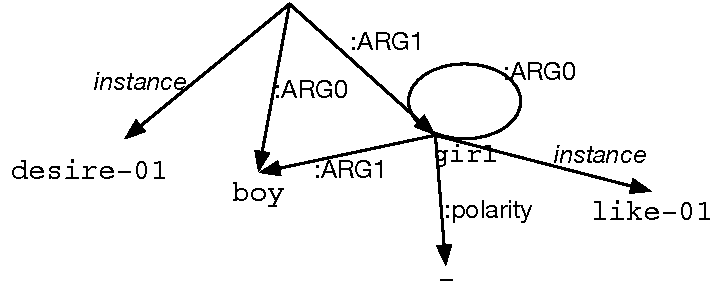
\includegraphics{images/AMRGraph.pdf}}
 \\
%  \hline    
% 2&\semr{}& % with inverse role!
%  \begin{lstlisting}[basicstyle=\scriptsize\ttfamily]
% (d desire-01 [:ARG0 (b boy [] @d),
%               :ARG1 (g girl [:ARG0-of (l like-01 [:polarity (- # [] @l),
%                                                   :ARG1 (^b # [] @l)] @g)] @d)])
%  \end{lstlisting}
%  \\
 \hline
2&\semr{}&
 \begin{lstlisting}[basicstyle=\scriptsize\ttfamily]
(d desire-01 [
    :ARG0 (b boy [] @d),
    :ARG1 (g girl [:*:ARG0 (l like-01 [:polarity (- # [] @l),
                                       :ARG1 (^b # [] @l),
                                       :ARG0 (^g # [] @l)] @g)] @d)])
 \end{lstlisting}
 \\
 \hline
3& \syntr{} &
 \begin{lstlisting}[basicstyle=\scriptsize\ttfamily,mathescape=false]
S(NP(D("the"),
     N("boy")),
  VP(V("desire"),
     NP(D("the"),
        N("girl"),
        SP(Pro("who"),
           S(VP(V("like"),
                Pro("me").pe(3).g("m"))).typ({"neg": true})))))
 \end{lstlisting}
 \\
 \hline
 \multicolumn{1}{|l|}{4}&
 \multicolumn{1}{|l}{English} & 
 \multicolumn{1}{|l|}{\texttt{The boy desires the girl who does not like him.}}\\
 \hline
 \end{tabular}
\caption{Representations used in the transformation of the \AMR{} structure shown in row~1 to the sentence shown in the last row. Row~2 is a representation of an internal Python representation of the \AMR{} once it is parsed. Row~3 is a Python expression (which happens to be also a legal JavaScript expression) that is the serialization of the internal representation created by the transformation process of \gophipy{}. This expression is used as input to \jsr{} to realize the English sentence shown in row 4.}
\label{tab:transformations}
\end{table}
\clearpage
% section amr_concepts (end)

\section{From \semr{}\\ to \syntr{}} % (fold)
\label{sec:semr2syntr}
As getting the \semr{} from an \AMR{} is a straightforward parsing job performed by recursive descent, the challenge is to transform the \semr{} to the \syntr{} (i.e. from the second to the third row of Table~\ref{tab:transformations}) which is detailed in this section.

The core of the system is conceptually simple:
a \semr{} (\SEMR{}) is transformed compositionally by means of lambda expression applications. Each concept in the dictionary is encoded as a lambda expression that returns an \syntr{} (\SYNTR{}). When concept is applied to its arguments (i.e. its roles) it creates a new \SYNTR{} corresponding to their composition. 

We illustrate this process with a simplistic example with the following Python definitions in which symbols starting with a capital letter are calls to a Python class constructor to create an internal Python structure corresponding to terminals and non-terminals in the classic constituent grammar notation. The constructors ignore \texttt{None} parameters.


\begin{lstlisting}[basicstyle=\footnotesize\ttfamily]
like_01 = lambda arg0,arg1: S(arg0,VP(V("like"),arg1))
boy     = lambda d,a: NP(optD(d),a,N("boy"))
girl    = lambda d,a: NP(optD(d),a,N("girl"))
\end{lstlisting}

\lstinline{like_01} is a lambda expression that corresponds to a constituency tree with \lstinline{S} as root; the first child is the subject given by \lstinline{arg0}, the second child is a \texttt{VP} tree with its first child being the verb \lstinline{like} and \lstinline{arg1} its second child, the object of the verb. When a lambda term is applied, a missing subject or object is indicated with the \lstinline{None} value. 

\lstinline{boy} and \lstinline{girl} are lambda expressions that build a constituency tree having \texttt{NP} as root with three children: the determiner, an adjective and the noun itself. To take into account optional parameters, we define the following function 
\begin{lstlisting}[basicstyle=\footnotesize\ttfamily]
    optD = lambda det : det if det!=None else D("the")
\end{lstlisting}
which inserts the definite determiner \lstinline{the} when \texttt{None} is specified.

Calling
\begin{lstlisting}[basicstyle=\footnotesize\ttfamily]
   like_01(boy(None,None),girl(D("a"),None))
\end{lstlisting}

creates a structure that can be pretty-printed as:
\begin{lstlisting}[basicstyle=\footnotesize\ttfamily]
S(NP(D("the"),
     N("boy")),
  VP(V("like"),
     NP(D("a"),
        N("girl"))))
\end{lstlisting} 

When an argument of a verb (e.g. \lstinline{give}) should be realized with a preposition, the lambda associated with the verb is defined as follows where \lstinline{pp} embeds the arguments in a prepositional phrase when it is not \lstinline{None}:
\begin{lstlisting}[basicstyle=\footnotesize\ttfamily]
give_01  = lambda arg0,arg1,arg2:S(arg0,VP(V("give"),arg1,pp("to",arg2)))
pp       = lambda prep, arg: PP(P(prep),arg) if arg!=None else None
\end{lstlisting}
Section~\ref{sub:python_implementation_of_lambda_application} gives more information about the Python implementation of this process.
 
In \AMR{}, argument values are given by the values of the roles which are recursively evaluated until they are given simple values found in the dictionary. \AMR{} concepts being the ones of \propbank{}, we created 7,912 verb entries of our dictionary by parsing the XML structures of \propbank{} frames to determine the arguments and used the annotated examples for determining the proper preposition to use. 
% (e.g. \texttt{for} in the \texttt{desire-01} concept in Table~\ref{tab:lambdas}).
We also parsed other \propbank{} XML entries for determining related 2,879 nouns and 1,352 adjectives. We also added about 33,300 nouns, adjectives, conjunctions and adverbs from an internal dictionary of our lab that did not appear in the entries of \propbank{}. Some pronouns and other parts of speech were added manually. 

If \AMR{} expressions were limited to \propbank{} concepts with frame arguments (i.e. $\texttt{:ARG}_{i}$) as roles then we could limit ourselves to this single application process, but there are many other \AMR{} peculiarities to take into account. We leave it to the reader to decide if these singularities are fundamental or just an artifact to ease annotation. Even then, we conjecture that a single and more uniform process would be preferable. We now describe how some of these special cases are handled. \gophi{} was developed on the AMR~2.0 corpus and we had hoped that some of these special cases could be limited in version 3.0. Unfortunately, it proved to be the inverse, many more \emph{constructions} were introduced in this version. 

\subsection{Polarity} % (fold)
\label{sub:polarity}
Negation in \AMR{} is indicated using a special role (\texttt{:polarity}) associated with \texttt{-}; this does not fit well with the lambda application process that we explained above. Fortunately, \jsr{} also uses this type of \emph{flag} to indicate that the current sentence should be negated. This process was borrowed from a similar mechanism in SimpleNLG~\cite{W09-0613} in which it is possible to mark a sentence as negated; the realization process then modifies the dependency structure to produce the negation of the original sentence. In \jsr{}, negation is indicated by specifying the \texttt{type} of sentence by adding \texttt{.typ("neg":true)} after the \texttt{S} constructor; this type of modification is called an \texttt{option} in \jsr{}. An example of this is shown in the row 3 of Table~\ref{tab:transformations}.  So when the application process encounters a \texttt{:polarity} role, it must keep track of the fact that an option should be added to this effect in the \syntr{}. This option \emph{trick} is also used in other cases, for example for generating interrogative sentences or adding modals. In some \AMR{}s, the \texttt{:polarity} role is also added to concepts that correspond to nouns or adjectives. Unfortunately this is not implemented by \jsr{}, so we had to check for these special cases.

% subsection polarity (end)
\subsection{Inverse Roles} % (fold)
\label{sub:inverse_roles}
Inverse roles (indicated by \texttt{-of} at the end of the role name) also do not easily fit in the lambda application process. They are introduced in \AMR{} mainly for keeping the focus on a single concept that is used in different frames. In our example of Table~\ref{tab:transformations}, \texttt{girl} is object in one frame and subject in another. Inverse roles can be quite delicate to process in the general case, but for our verbalization context we decided to systematically introduce a relative clause. After trying some alternatives, we resorted to a \emph{hack}: we transform the original \AMR{} containing inverse roles into one that only uses active roles but flagged to indicate to the realizer that a relative clause should be introduced. Table~\ref{tab:transformations} shows an example of this transformation between rows~1 and 2 where a \texttt{:ARG0-of} has been transformed into a \texttt{:*:ARG0} role with an explicit \texttt{:ARG0} role added in the inner concept. This approach is appropriate for \emph{short} \AMR{}s, but it often results in embedded relatives for \emph{deep} ones that are almost unreadable.

% subsection inverse_roles (end)

\subsection{Non-Core Roles} % (fold)
\label{sub:non_core_roles}
As described in the AMR Guidelines~\cite{AMR-Guidelines}, there are 46 other \emph{non-core} roles such as: \texttt{:domain}, \texttt{:mod} etc., each of which must be dealt specifically. But the basic principle remains the same, each AMR associated with a role is evaluated recursively and its \syntr{} is added to the deep structure of the current concept most often at the end of the values of the core roles. For example, for a \texttt{:destination}, we add a prepositional phrase starting by preposition \texttt{to}.  In other cases, e.g. \texttt{:polite +}, then the word \texttt{Please} is added at the start of the syntactic structure. In an AMR, the \texttt{:wiki} role is used to disambiguate named entities, we use its value as the target of an HTML link that the system generates.

% subsection non_core_roles (end)
\subsection{Special concepts} % (fold)
\label{sub:special_concepts}
Some \emph{special} concepts appear quite frequently and many new ones were added in the release 3.0 of \AMR{}, but we did not manage to deal with them using the above framework.
\begin{description}
 \item[\texttt{amr-unknown}] is most often used for annotating an interrogative form; although intuitively this is convenient for the annotator and easy for a human to understand, automatically finding the appropriate form of interrogation is quite difficult because it depends on the enclosing role: e.g. if it appears as the value of an \texttt{:ARG0} or \texttt{:ARG1} then the question should start with \texttt{who}, if it appears as an argument of \texttt{:polarity}, then it should be a yes-or-no question, etc. Fortunately, \jsr{} has options to transform affirmative into interrogative forms of different types, so in most cases, it is only a matter of adding the right option depending on the context. But there are still cases that are not dealt with correctly in the system. A closer examination of the use of \texttt{amr-unknown} revealed that this \emph{vague} concept seemed to have been interpreted in diverse ways by different annotators.
 \item[\texttt{date-entity}] has more than ten specific roles which have to be taken into account to represent time, date, day-period and even calendar type.
 \item[\texttt{government-organization}] encodes the name of different governmental entities that should be realized in specific ways to match their official names.
 \item[\texttt{have-degree-91}] indicates the comparison between two entities and often induces dependencies between structures of different roles. For example, a comparative is annotated using different roles for the domain, the attribute, the degree, the object of the comparison and a possible reference to a superset. Finding appropriate verbalizations for all these cases proved quite tricky but essential as this concept is often used.
 \item[\texttt{have-polarity-91}] is a reification (see Section~\ref{sub:verbalization}) of polarity with a specific use of \texttt{:ARG2}.
 \item[\texttt{have-quant-91}] which serves to mark a relation between an owner and specific types of quantifiable goods for certain goals.
 \item[\texttt{have-rel-role-91}] indicates the relation between two entities (often child concept of \texttt{person}, another special concept) and the type of relation (e.g. \texttt{father}, \texttt{sister},...) all using different roles.  This also needs specific processing to get colloquial reading. For example, \lstinline{my wife} is encoded as
 \begin{lstlisting}
 (p / person :ARG0-of (h / have-rel-role-91 :ARG1 (i / i) :ARG2 (w2 / wife)))
 \end{lstlisting}
 otherwise it would be verbalized as \texttt{the person who is relation of wife with me}.
 \item[\texttt{hyperlink-91}] is used to connect a URL to regular text with specific roles values.
 \item[\texttt{multisentence}] combines annotations and linking instances between many sentences. Verbalizing them is a simple matter of creating as many sentences as there are roles.
 \item[\texttt{ordinal-entity}] to deal with some specific ways of verbalizing ordinal numbers: e.g. \texttt{last} for -1, \texttt{second to last} for -2, etc.
 \item[\texttt{*-quantity}] there are about a dozen types of quantities, for which the roles \texttt{:quant} and \texttt{:unit} must be combined appropriately (using the value of the quantity as determiner for the unit when this value is a numeric value).
\end{description}

We did not manage to find a systematic handling of these special cases, we are left under the impression that they are a symptom of some design deficiencies in the original \AMR{} formalism.

\subsection{Pronoun generation} % (fold)
\label{ssub:pronoun_generation}
Variables in \AMR{} enable the coreference between entities and create a graph between elements that could otherwise be considered as a tree. Although quite intuitive for the annotator, it proved to be quite intricate to generate the appropriate pronoun. Although we can deal properly with usual cases, there are still pending problems. Some of them have to do with the fact that, by design, \AMR{} abstract important grammatical information such as gender and number; for example, \emph{Steffi Graf} is referred to using \texttt{he} or \emph{Yankees} is used as singular (see Figure~\ref{fig:web-gophipy}). English pronouns also are different when used as nominative (\texttt{:ARG0} $\rightarrow{}$ \texttt{I})  or as accusative (\texttt{:ARG1}  $\rightarrow{}$ \texttt{me}). But this \emph{trick} does not always work because it depends on the argument structure of the concept and the fact that the subject or object is animate or not, an information that is not available because it would imply understanding the comments in the \propbank{} file.
% subsubsection pronoun_generation (end)

\subsection{Passive and other peculiarities} % (fold)
\label{sub:passive}
\AMR{} does not indicate if the sentence should be realized as a passive. Instead annotators seem to rely on a convention that a verb with a subject, usually indicated by \texttt{:ARG0}, is used with an \texttt{:ARG1} instead. This fact must be checked before any other processing because passive is used extensively in English, especially in the news genre often encountered in the annotated corpora. Other special cases that must be checked are imperative and \emph{yes or no question} that use the \texttt{amr-choice} special concept as \texttt{:ARG1}. Moreover the \AMR{} editor provide some \emph{shortcuts} that are expanded in the resulting \AMR{}. For example, \texttt{cause-01} is expanded as an inverse role, that we have to check and \emph{un-expand} to produce a more readable sentence. Many named entities\footnote{A list is given at \url{https://www.isi.edu/~ulf/amr/lib/ne-types.html}} followed by a proper name are explicitly given in the \AMR{}, but only the proper noun is written out in the text (see \emph{Yankees} in Figure~\ref{fig:web-gophipy}). \gophipy{} checks for many of these in order to simplify the output.
% subsection passive (end)

% subsection special_concepts (end)
\subsection{Verbalization and Reification} % (fold)
\label{sub:verbalization}
\AMR{} is oblivious to verbalization, see our example of Table~\ref{ex:paper} for which \texttt{The boy desires} and \texttt{The desire of the boys} are annotated using the single concept \texttt{desire-01}. Using tables provided on the ISI website\footnote{Resource list section at \url{https://amr.isi.edu/download.html}} for helping annotators, we added some verbalization information to the dictionary which is used to nominalize a verb when it does not have a subject.

Roles can sometimes be used as a concept, a process called \emph{reification} e.g. \texttt{:location} is reified as \texttt{be-located-at-91}. This is used to indicate that the focus of the sentence is the locating process itself instead of the object being located or to the location itself. Mapping tables between roles and their reifications are given on the ISI website and we adapted them for our context. Our implementation \emph{dereifies} the cases identified by Goodman~\cite{Goodman:2019} before processing the \AMR{}.

% subsection verbalization (end)
\subsection{Unknown Role or Concept} % (fold)
\label{sub:unknown_role_or_concept}
When an unknown concept is encountered, we use the fact that \AMR{} is English centric and that English morphology is relatively simple, at least compared to French and German. So we merely use the name of the concept, after removing dashes or the frame number, as the word to add to the sentence. When an unknown role is encountered, the corresponding \AMR{} value is added at the end of the current constituent, ignoring the name of the role.

% subsection unknown_role_or_concept (end)
\subsection{Conclusion} % (fold)
\label{sub:conclusion}
Although the basic principle for creating an \AMR{} verbalizator is a simple $\beta$-reduction of lambda forms, there are (too~?) many special cases that do not fit well within the declarative approach to the transformation from \semr{} to the \syntr{}.

An important limitation of our current implementation is the fact that we do not take lexical ambiguity into account, so if a concept corresponds in the dictionary either to a verb or to a noun, we consider only the verb entry. Some \AMR{} examples (e.g. given in \cite{Bos2019}) include the part of speech in the name of the concept e.g. \texttt{check.v.01} or \texttt{check.n.01} instead of \texttt{check-01}, but our corpora do not provide this information.

% subsection conclusion (end)

% section from_semr_to_syntr (end)

\section{Implementation} % (fold)
\label{sec:implementation}

The whole system is written in Python (4,000 lines), of which more than 1,000 for dealing with \emph{special cases} described in sections~\ref{sub:polarity} to \ref{sub:special_concepts}.  The parsing of the \propbank{} XML files generates a 58,000 lines dictionary. The final realization of the English sentence is produced by \jsr{} as a \systeme{Node.js} module taking as input the \syntr{}.

To develop \gophipy{}, we used the same examples used for developing \gophi{}: 268 examples from the AMR Guidelines~\cite{AMR-Guidelines} and the 826 examples from the AMR Dictionary~\cite{AMR-Dictionary}. These \AMR{}s are usually short sentences that combine a few concepts for didactic purposes and are designed to cover most of the annotation cases; they are thus ideal for developing a system, even though most sentences in the \emph{real} corpora are much longer and combine diverse roles in a single \AMR{}. Release 3.0 of \AMR{} has introduced a subset of the corpus (8027 AMRs)  annotated at the document level for coreference, implicit role reference, and bridging relations.

We recall that our goal is not to reproduce verbatim the original sentence, but to give a literal reading of the \AMR{} in which all verbs are generated at the present tense and in the active voice; all nouns are singular with a definite determiner. Given the fact that the original sentences usually have a great variation in number, tense (some informal sentences are even encountered, see Table~\ref{ex:dh_in_ae}), it is expected that the BLEU scores between the reference and our \emph{standardized} output will not be high. Moreover, \gophipy{} also generates an HTML link when  a \texttt{:wiki} role is used in an AMR (see the bottom part of Figure~\ref{fig:web-gophipy}).

\gophipy{} produced a sentence for all \AMR{}s of our development, test and training examples:  corpora available at the ISI website~\footnote{\url{https://amr.isi.edu/download.html}} and the ones from the AMR 3.0 Distribution~\cite{AMR-Release3} 
%(see Table~\ref{tab:corpora} for more details). 
\gophipy{} run on a MacBook laptop (1.2~GHz without GPU!) is quite fast: a few milliseconds of CPU and about 7 ms of real time per sentence. Of course, longer sentences take more time to verbalize, but it is still quite fast compared to other statistical systems which take seconds for computing an English sentence even after a longer initial loading phase. These timings are for Python to parse the AMR and producing the \syntr{}, \jsr{} is also almost instantaneous.
The generated sentences are systematically longer than the reference sentence, between 15\% up to 70\% longer, for a mean of 38\%.

We also developed a web server\footnote{\url{http://rali.iro.umontreal.ca/amr/python/current/export/cgi-bin/amrVerbalizer.cgi}}, also written in Python, that displays a web page (see Figure~\ref{fig:web-gophipy}) in which a user can edit an AMR. The AMR is then transformed and its English realization is generated by an instance of \jsr{} integrated in the response web page itself. This setup allows the web links generated by \jsr{} to be clicked directly from this web page (see the words \emph{Yankees} in the right part of the figure). This example (numbered isi\_0001.12) taken from the AMR Dictionary gives as a reference sentence: \emph{The boy doesn't think the Yankees will win.}\footnote{This sentence is reproduced verbatim by \spring{}.} in which the negation is not given the same scope in the reference and in the \AMR{}. This is a case in which an \AMR{} verbalizer could have helped catch this type of discrepancy because the annotator could have noticed that the generated sentence from the \AMR{} has a slightly different meaning than the original sentence, so it should be double-checked.

% trick taken from http://texblog.net/latex-archive/graphics/includegraphics-top-align/
\begin{figure}[ht]
  \centering
    \fbox{\begin{minipage}[t]{0.48\textwidth}
            \vspace{0pt}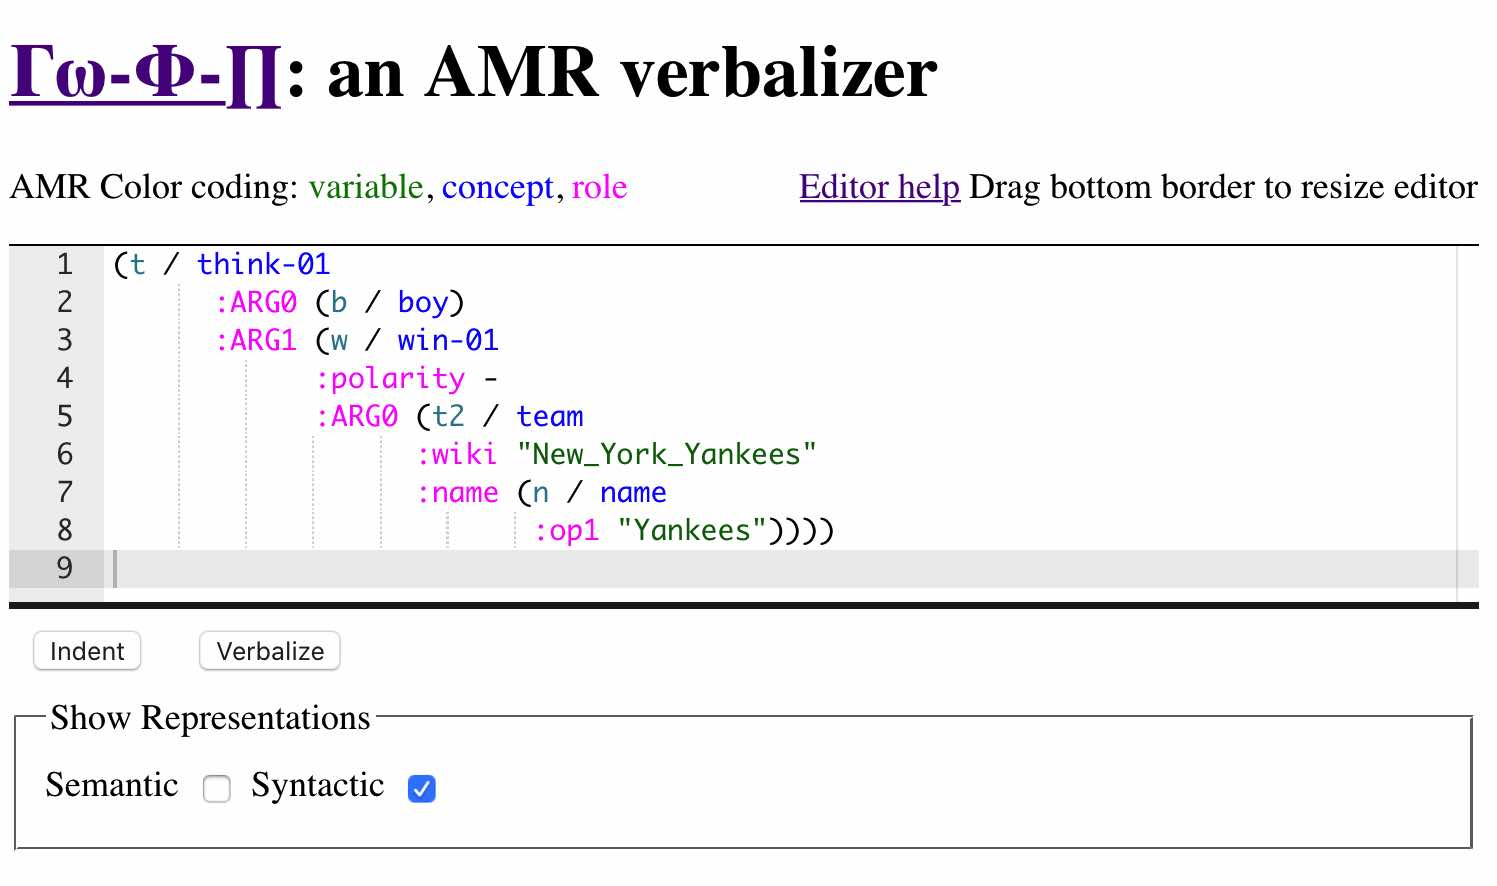
\includegraphics[width=\textwidth]{images/web-gophipy-1.jpg}
        \end{minipage}}
    \hfill
    \fbox{\begin{minipage}[t]{0.48\textwidth}
            \vspace{0pt}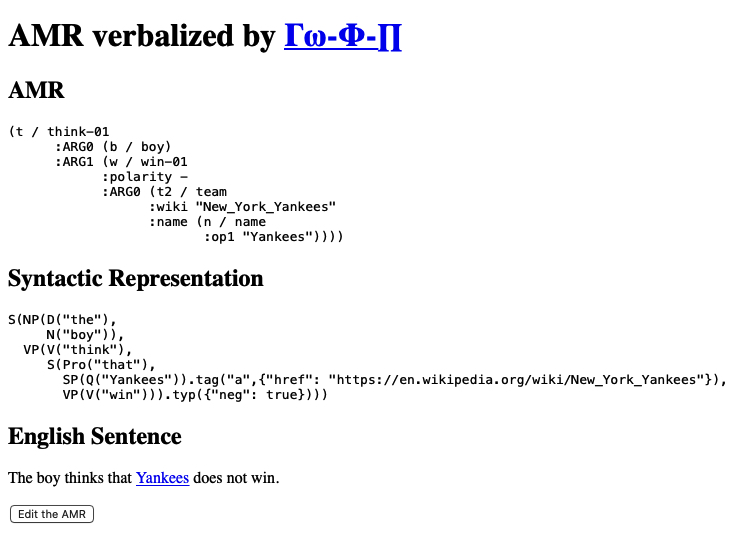
\includegraphics[width=\textwidth]{images/web-gophipy-2.jpg}
        \end{minipage}}
  \caption{Web interface to the verbalizer. The input page on the left shows an editor with a special \emph{mode} for editing AMRs; intermediate representations can also be requested with the checkboxes at the bottom, only \SYNTR{} is chosen here. The right part shows the corresponding \SYNTR{} (in indented form) and the realized sentence created by the embedded \jsr{} module in the webpage.}
  \label{fig:web-gophipy}
\end{figure}
% section implementation (end)
%
\clearpage{}
\section{Evaluation} % (fold)
\label{sec:evaluation}

\AMR{} generation outputs up to now have been evaluated either by means of BLEU scores \cite{DBLP:conf/naacl/FlaniganDSC16,DBLP:conf/inlg/PourdamghaniKH16,bevilacqua-etal-2021-one} and by means of pairwise comparisons~\cite{SemEval2017-T9-Desc}. But unfortunately these metrics are not very useful for helping the development or the improvement of a symbolic system.

\subsection{Development Evaluation} % (fold)
\label{sub:development_evaluation}

So in order to keep track of the \emph{progress} of our system, we devised a crude metric
using the scale shown in Table~\ref{tab:evaluation-scale}. During the course of our development, we manually evaluated a small subset to measure the adequacy of the generated sentence for the intended purpose, that is, helping an annotator to check if the proper concepts and roles have been chosen in the annotation. This evaluation scale helped us focus on the most frequent drawbacks of the system. 

\begin{table}[ht]
\centering
 \begin{tabular}{ll}
  4 & Perfect translation of all concepts of the \AMR{} and acceptable English formulation\\
  3 & Translation correct, but bad English formulation\\
  2 & Translation correct, but English barely understandable\\
  1 & Gibberish in the English\\ 
    & or missing important information from the \AMR{} or bad meaning conveyed\\
  0 & Error in the parsing, translation or generation (not encountered anymore!)\\
 \end{tabular}
\caption{Scale used for the evaluation of the results}
\label{tab:evaluation-scale}
\end{table}

We do not give here the results on the development corpora, but instead we focus on the results obtained on a random sample 25 \AMR{}s taken from the six test sets of the AMR 3.0 Distribution~\cite{AMR-Release3}. In order to focus on \emph{interesting} \AMR{}s, we removed those having less than 5 lines; They account for about 20\% of all cases and are often only auxiliary informations such as dates, amounts, author names, etc. In doing so, we penalize the scores of the systems which almost always realize these \texttt{short} \AMR{}s perfectly. We feel that the generation challenge sits in the realization of complex \AMR{}s, otherwise a plain formatter would be sufficient.

% (see Section~\ref{sub:description_of_the_corpora} for more details).
Table~\ref{tab:eval-statistics} shows the score we gave for the both \gophipy{} and \spring{}~\cite{bevilacqua-etal-2021-one}. As the generation of web links is systematic, HTML tags were removed from the generated text before the evaluation. Comparison with the reference sentence is not taken into account in this evaluation as the generated verbs are always conjugated at the present tense, the nouns are always singular and the determiners always definite. 

\spring{} is the clear winner not only in terms of BLEU scores, but also in the number of perfect translations: in fact, in some cases, the \spring{} formulations were more fluent than the reference one. 82\% of the formulations produced by \gophipy{} and 87\% by \spring{} were considered as useful (scores 3 and 4). 12\% of the \gophipy{} formulations had a very bad English formulation namely because it is strictly compositional and thus it creates complex sentences with many subordinates that mirror the nested nature of the \AMR{}. In some cases, this makes it very hard to see what parts of a sentence relate to another.

Our crude scale assign 1 for two different reasons: as \gophipy{} explicits the input \AMR{}, it never forgets to render any information, unless there is a bug in the system, so this score is only given for very bad formulation. 
\begin{table}[ht]
\centering
\begin{tabular}{|l|r|r|r|rrrrr|}
\hline
\multicolumn{1}{|c}{System}&
\multicolumn{1}{|c|}{BLEU}&
\multicolumn{1}{|c}{CPU secs}&
\multicolumn{1}{|c}{Mean}&
\multicolumn{1}{|c}{4} &
\multicolumn{1}{c}{3} &
\multicolumn{1}{c}{2} &
\multicolumn{1}{c}{1} &
\multicolumn{1}{c|}{0} \\
\hline
\gophipy{} &  7.00 &   1.7 & 3.14 &  54 & 70 & 19 &  7 & 0 \\
\spring{}  & 34.62 & 264.0 & 3.60 & 128 &  3 &  0 & 19 & 0 \\
\hline
\end{tabular}
\caption{Statistics of the manual evaluation scores on a sample of 25 \emph{long} AMRs taken from each the six split/test corpora of Release 3.0 of AMR for \gophipy{} and \spring{}. The second column gives the BLEU scores. The third column gives the mean score over all 150 manual evaluations of this corpus; columns 4 to 8 give the number of sentences that were given the corresponding score between 4 and 0.}
\label{tab:eval-statistics}
\end{table}

As this bad formulation problem was never encountered for \spring{}, this score was given in 12\% of cases when some information was missing or when the sentence did not convey appropriately the information found in the \AMR{} input.
Here is more detailed analysis of the these cases which are relatively hard to spot because the generated text is so fluent that one must be very careful in checking these translations:
\begin{itemize}
    \item 6 cases of missing information such as number, dimension and even a case of missing \texttt{not};
    \item creation of \emph{strange} words: \emph{prostitiators}, \emph{go-go};
    \item 9 cases of change in meaning: e.g. \emph{China is stronger than Korea}, but the \AMR{} says the inverse
    \item in the case of multi-sentence, the \texttt{snt\emph{i:}} roles are sometimes not sorted in the \AMR{}, so \spring{} follows the order of the input and not of the \texttt{snt\emph{i:}}, this problem could probably be fixed during the \AMR{} linearization step;
\end{itemize}

The only clear advantage of \gophipy{} over \spring{} is in computation time: it takes less than two seconds on a commodity laptop while \spring{} needs more than four minutes on high-power machine with a GPU and many gigabytes of memory.

% section evaluation (end)

\section{Future Work} % (fold)
\label{sec:future_work}

This paper has described a symbolic \AMR{} verbalizer that shows that the approach is viable and fast. There is still work to do on many aspects.

% First a more systematic manual evaluation should be performed because currently only the author of the system has evaluated the output using a rough scale. The author was probably a bit too lenient at times... It would be interesting to use the evaluation protocol developed for \emph{SemEval-2017}, but this would imply recruiting many volunteers who are willing to understand the \AMR{} enough to appreciate if the generated text is appropriate. At SemEval, this evaluation was performed by the authors of the systems who were all familiar with the \AMR{} formalism. Similar scores were obtained by taking into account all output of systems or ignoring the scores that system developers gave to output of their own systems.
%
% There are still many missing concepts and roles, most of which would imply adding or correcting dictionary entries. Currently the system outputs warnings when unknown concepts and roles are encountered, so this process would imply collecting those warnings. It would also be helpful for annotators to realize that they have \emph{invented} new roles or concepts.

\gophipy{} should take lexical ambiguity into account. Currently if the same character string can refer to a verb, a noun or an adjective such as \texttt{war} or \texttt{good}, the system chooses the first fit in the above order. When this is not appropriate, we manually removed the \emph{bad} entry (e.g. the verb entry for \texttt{war} and the noun entry for \texttt{good}). This process gives acceptable results most of the time, but it should be revised using a better linguistically justified process.

Currently an \AMR{} is verbalized as a single sentence, except in the case of a \texttt{multisentence}; thus sentences are sometimes long-winded and even repetitious. This is due to the depth-first traversal of the graph and also because relative sentences are used most of the time for inverse roles.  The nominalization should be better integrated and could sometimes help in reducing the verbosity of the generated text. A better use of pronouns could also help shorten or split long sentences.

Although the system has been tested on all available \AMR{} corpora, the implementation is still a bit shaky: it involves feeding the output of a Python system (\gophipy{}) into \jsr{}, a Javascript module. An error in the input of \jsr{} must sometimes be linked back to the Python system (often an error in the generated dictionary).
This process should be streamlined even though we could run many ten of thousands of examples without any problem.

It might also be interesting to revisit the starting point of the transformation: there has been extensive work for generating text from \fol{} which can be systematically generated from \AMR{}. It would probably be worth a try to revisit this aspect that we gave up perhaps a bit too soon.

It would also be interesting to try to use machine learning techniques to develop the transformation rules between the \semr{} and \syntr{}, hoping that the process will learn how to cope with many of the special cases. It would probably also solve some of the \emph{hallucination} problems encountered by \spring{}.

\subsection{Suggestions for \AMR{} Developers} % (fold)
\label{sub:suggestions_for_amr_developers}

We also think that \AMR{} developers should benefit from taking a \emph{generative} view: we have observed  a recent tendency to add new concepts and roles as a way to ease the annotation, but this makes the generation process more complex. This proliferation of new \emph{primitives} also makes the use of machine learning techniques more difficult as there are only very few instances (often only one) of each in the training material, although \spring{} manages to generates excellent texts most of the time.   We suggest that the \AMR{} developers try to limit the number of roles to the bare minimum as they have successfully done with the syntactic peculiarities. The annotators should also limit the use of inverse roles, not only because they are difficult to verbalize by our system~$\ddot\smile$, but because they do not seem to add to the semantics, especially when inverse roles are composed (i.e. the inverse role of a concept that is itself used in an inverse role). The problem has even been exacerbated in Release 3.0 of the AMR, because the release notes claim that the \emph{AMR deepening} is an important feature of this release with hundreds of new frames, some of them very specialized such as \texttt{read-between-lines-09} or \texttt{take-with-grain-of-salt-36}.

Although Bos has shown that the \texttt{meaning} of \AMR{}s can be expressed in first-order logic, it would be interesting to develop a theory of \emph{non-core roles} (e.g. why are some roles important or necessary ?) and their relations with language or other NLP applications. Such a theory would have been helpful for us when developing our system; for example, \texttt{:ARG$_i$} roles have been studied for a long time and their meaning is relatively well defined, so their implementation for generation is relatively \emph{clean}. Many other roles do not seem to have well-defined semantics (e.g. \texttt{:mode}, \texttt{:manner}, \texttt{:time} which depends on the context of use, etc.), some relations (e.g. comparisons) are expressed in many different ways in the corpus. A much more systematic coding of \AMR{}s would surely simplify the analysis of their meaning and help in their use in future NLP applications.

The current \AMR{} corpus is interesting in its diversity: news articles, biology texts, novels, tutorial examples, informal (even vulgar!) examples and contrived texts that \emph{linguists love}\footnote{See example isi\_0002.315: \texttt{Buffalo buffalo Buffalo buffalo buffalo buffalo Buffalo buffalo.}}. This shows that \AMR{} can convey almost any kind of text, but then it makes it difficult for system developers to focus on specific aspects. So it might be interesting to annotate texts that will target specific application areas.
% subsection suggestions_for_amr_developers (end)

% section future_work (end)

\section{Conclusion} % (fold)
\label{sec:conclusion}

We have described \gophipy{} a text generator from \AMR{} input. It is a proof of concept of a feasible symbolic approach to \AMR{} generation that takes advantage of the fact that \AMR{} is a structured input that can serve as a plan for the output text. We have shown the interest of generating constituency structures instead of full sentences that can be obtained systematically from them. We have also shown that our previous system \jsr{} can be a useful intermediary especially for producing variations of structure.

% section conclusion (end)

\section*{Acknowledgements} % (fold)
\label{sec:acknowledgements}
We thank Fabrizo Gotti for many fruitful discussions and suggestions, for helping with the evaluation and for installing the ISI AMR to English generator on our servers. We thank Philippe Langlais who made detailed suggestions for improving the organization of the paper. 
% section acknowledgements (end)
\bibliographystyle{plain}
\bibliography{GoPhi}

\newpage
\section{Appendix} % (fold)
\label{sec:appendix}
\subsection{Some \AMR{}s with output produced by some generators} % (fold)
\label{sub:_amr_s_with_generated_systems}

The following tables give a few \AMR{} structures, the corresponding reference English sentences and the sentences produced by 6 different generators to give a perspective on the current state of our system and that of other generators:
\begin{description}
 \item[\gophipy{}] System described in this paper, we indicate in parentheses the development evaluation score given to this sentence;
 \item[\spring{}] System described by Bevilacqua et al.~\cite{bevilacqua-etal-2021-one} and run using a Google Colaboratory machine according to the instructions given on the implementation site \footnote{\url{github/SapienzaNLP/spring}}
 \item[\jamr{}] Pretrained generation model of Flanigan~\cite{DBLP:conf/naacl/FlaniganDSC16} used \emph{out of the github} with the provided Gigaword corpus 4-grams;
 \item[\isimt{}] System developed by ~\cite{DBLP:conf/inlg/PourdamghaniKH16} and made available at the ISI website as the \texttt{AMR-to-English generator}\footnote{\url{https://www.isi.edu/projects/nlg/software_1}};
 \item[Generate] Output of the \texttt{generate} button in the AMR Editor~\cite{AMR-Editor};
 \item[Baseline] Our own baseline generator (20 lines of Python) that merely does a top-down recursive descent in the AMR structure and outputs the concepts encountered. If an \texttt{:ARG0} is present, it is output before the root concept in order to try to keep the subject in front of the verb. \texttt{not} is added when a negative polarity is encountered and \texttt{that} is inserted in the case of an inverse role.
\end{description}
% subsection _amr_s_with_generated_systems (end)
\noindent
%%  le contenu des lstlisting doit être "escapé" car il est utilisé dans une macro (OUACHE)!!!
\begin{table}[ht]
\begin{tabular}{|p{1in}|p{5.25in}|}%
\hline
\multicolumn{2}{|p{6in}|}{
\begin{lstlisting}^^J
(f \/ fire-01^^J
\ \ \ \ \ \ :ARG0 (a \/ aircraft-type^^J
\ \ \ \ \ \ \ \ \ \ \ :wiki "Mikoyan-Gurevich_MiG-25"^^J
\ \ \ \ \ \ \ \ \ \ \ :name (n \/ name^^J
\ \ \ \ \ \ \ \ \ \ \ \ \ \ \ \ :op1 "MiG-25"))^^J
\ \ \ \ \ \ :ARG1\ (m / missile^^J
\ \ \ \ \ \ \ \ \ \ \ :source (a2 \/ air)^^J
\ \ \ \ \ \ \ \ \ \ \ :direction (a3 \/ air))^^J
\ \ \ \ \ \ :destination (a4 \/ aircraft-type^^J
\ \ \ \ \ \ \ \ \ \ \ :wiki "General_Atomics_MQ-1_Predator"^^J
\ \ \ \ \ \ \ \ \ \ \ :name (n2 \/ name^^J
\ \ \ \ \ \ \ \ \ \ \ \ \ \ \ \ :op1 "Predator")))^^J
\end{lstlisting}
}\\
\hline
\emph{Reference}&  The MiG-25 fired an AAM at the Predator.\\\hline
\gophipy{} (4)&{\raggedright \textless{}a href='https://en.wikipedia.org/wiki/Mikoyan-Gurevich\_MiG-25'\textgreater{} MiG-25\textless{}/a\textgreater{} fires the missile from the air to the air to \textless{}a href='https://en.wikipedia.org/wiki/General\_Atomics\_MQ-1\_Predator'\textgreater{} Predator\textless{}/a\textgreater{}}\\\hline
\spring{}&The MiG-25 fired an AAM at the Predator.\\\hline
\jamr{}&mig-25 mikoyan-gurevich\_mig-25 general\_atomics\_mq-1\_predator predator aircraft fired the missiles in the air in the air
\\\hline
\isimt{}& fire aircraft-type :wiki mikoyan-gurevich\_mig mig-21 missiles from the air to air to aircraft-type :wiki general\_atomics\_mq-1\_predator predator\\\hline
\emph{Generate}& fire missile air from air to\\\hline
\emph{Baseline}&aircraft-type "Mikoyan-Gurevich\_MiG-25" name "MiG-25" fire missile air air aircraft-type "General\_Atomics\_MQ-1\_Predator" name "Predator"\\
\hline
\end{tabular}
\caption{AMR and their realization with different systems (ex: \texttt{isi\_0002.701})}
\label{ex:isi_0002.701}
\end{table}

\noindent
\begin{table}[ht]
\begin{tabular}{|p{1in}|p{5.25in}|}%
\hline
\multicolumn{2}{|p{6in}|}{
\begin{lstlisting}^^J
(k / know-01^^J
\ \ \ \ \ :polarity -^^J
\ \ \ \ \ :ARG0\ (i\ /\ i)^^J
\ \ \ \ \ :ARG1\ (t\ /\ truth-value^^J
\ \ \ \ \ \ \ \ \ \ :polarity-of\ (s\ /\ straight-05^^J
\ \ \ \ \ \ \ \ \ \ \ \ \ \ \ :ARG1 (h / he))))^^J
\end{lstlisting}
}\\\hline
\emph{Reference}&   IDK if he's str8.\\\hline
\gophipy{}(4)&I do not know whether he is straight. \\\hline
\spring{}&I don't know if he's str8.\\\hline
\jamr{}&i know that he is straight -\\\hline
\isimt{}&I not know truth-value that was noted straight he.\\\hline
\emph{Generate}& i don't know truth-value :polarity-of straight from him.\\\hline
\emph{Baseline}&i not know truth-value straight he\\
\hline
\end{tabular}
\caption{AMR and their realization with different systems (ex:\texttt{isi\_0002.691})}
\label{eX:isi_0002.691}
\end{table}

\noindent
\begin{table}[ht]
\begin{tabular}{|p{1in}|p{5.25in}|}%
\hline
\multicolumn{2}{|p{6in}|}{
\begin{lstlisting}^^J
(b / bind-01^^J
\ \ \ :ARG1\ (s\ /\ small-molecule^^J
\ \ \ \ \ :wiki\ -^^J
\ \ \ \ \ :name\ (n\ /\ name^^J
\ \ \ \ \ \ \ \ \ \ :op1\ "TKI258"))^^J
\ \ \ :ARG2\ (e\ /\ enzyme^^J
\ \ \ \ \ :wiki\ "Fibroblast_growth_factor_receptor_1"^^J
\ \ \ \ \ :name\ (n2\ /\ name^^J
\ \ \ \ \ \ \ \ \ \ :op1\ "FGFR1")^^J
\ \ \ \ \ :ARG1-of\ (k\ /\ knock-down-02)^^J
\ \ \ \ \ :ARG2-of\ (m\ /\ mutate-01^^J
\ \ \ \ \ \ \ \ \ \ :value\ "V561M"))^^J
\ \ \ :ARG4\ (b2\ /\ binding-affinity-91^^J
\ \ \ \ \ \ :ARG1\ (i2\ /\ inhibitor-constant)^^J
\ \ \ \ \ \ :ARG2\ (a\ /\ approximately^^J
\ \ \ \ \ \ \ \ \ \ \ :op1\ (c\ /\ concentration-quantity^^J
\ \ \ \ \ \ \ \ \ \ \ \ \ \ \ \ :quant\ 35^^J
\ \ \ \ \ \ \ \ \ \ \ \ \ \ \ \ :unit\ (n3\ /\ nanomolar))))^^J
\ \ \ :ARG4\ (t\ /\ tight-05)).^^J
\end{lstlisting}
}\\\hline
\emph{Reference}&  TKI258 binds tightly to the FGFR1 KD V561M (Ki ~ 35 nM)\\\hline
\gophipy{} (3)&{\raggedright Is bound TKI258 \textless{}a href='https://en.wikipedia.org/wiki/Fibroblast\_growth \_factor\_receptor\_1'\textgreater{}FGFR1 that knocks down that mutate V561M\textless{}/a\textgreater{} with the binding-affinity inhibitor constant approximately nanomolar 35 tight.}\\\hline
\spring{}&TKI258 binds tightly to the FGFR1 KD V561M (K\textless{}sub\textgreater{}2\textless{}/sub\textgreater{} ~ 35 nM).\\ \hline
\jamr{}&inhibitor-constant binding-affinity approximately 35 nanomolar tightly binds tki258 - with knock-down mutating v561m fgfr1 fibroblast\_growth\_factor\_receptor\_1\\\hline
\isimt{}&bound small-molecule :wiki doesn't tki258 enzyme :wiki fibroblast\_growth\_factor\_receptor\_1 fgfr1 by knock-down of mutating v561m to binding-affinity inhibitor-constant approximately 35 concentration-quantity nanomolar to tight\\\hline
\emph{Generate}& bind that was knock-downed and was mutated tight .\\\hline
\emph{Baseline}&bind small-molecule - name "TKI258" enzyme "Fibroblast\_growth\_factor\_receptor\_1" name "FGFR1" knock-down mutate "V561M" binding-affinity inhibitor-constant approximately concentration-quantity 35 nanomolar tight\\
\hline
\end{tabular}
\caption{An \AMR{} for a biology text as generated by different systems (ex: \texttt{isi\_0002.786})}
\label{ex:isi_0002.786}
\end{table}

\noindent
\begin{table}[ht]
\begin{tabular}{|p{1in}|p{5.25in}|}%
\hline
\multicolumn{2}{|p{6in}|}{
\begin{lstlisting}^^J
(k / know-01^^J
\ \ \ \ \ :ARG0\ (i\ /\ i)^^J
\ \ \ \ \ :ARG1\ (t\ /\ thing^^J
\ \ \ \ \ \ \ \ \ \ :ARG0-of\ (c\ /\ cause-01^^J
\ \ \ \ \ \ \ \ \ \ \ \ \ \ \ :ARG1\ (c2\ /\ cross-02^^J
\ \ \ \ \ \ \ \ \ \ \ \ \ \ \ \ \ \ \ \ :ARG0\ (c3\ /\ chicken)^^J
\ \ \ \ \ \ \ \ \ \ \ \ \ \ \ \ \ \ \ \ :ARG1\ (r / road)))))^^J
\end{lstlisting}
}\\\hline
\emph{Reference}&  I know why the chicken crossed the road.\\\hline
\gophipy{} (4)&I know the thing that causes that the chicken crosses the road.\\\hline
\spring{} & I know why the chicken crossed the road.\\ \hline
\jamr{}&i know the things that cause the chicken cross the road\\\hline
\isimt{}&know why the chicken cross the road? \\\hline
\emph{Generate}& I know thing that caused chicken crossing road .\\\hline
\emph{Baseline}&i know thing cause chicken cross road\\
\hline
\end{tabular}
\caption{AMR and their realization with different systems (ex: \texttt{isi\_0002.766})}
\label{ex:isi_0002.766}
\end{table}

\noindent
\begin{table}[ht]
\begin{tabular}{|p{1in}|p{5.25in}|}%
\hline
\multicolumn{2}{|p{6in}|}{
\begin{lstlisting}[basicstyle=\scriptsize\ttfamily]^^J
(a / and^^J
\ \ \ \ \ :op1 (r / remain-01^^J
\ \ \ \ \ \ \ \ \ \ \ :ARG1\ (c / country :wiki "Bosnia_and_Herzegovina"^^J
\ \ \ \ \ \ \ \ \ \ \ \ \ \ \ \ \ \ :name (n / name :op1 "Bosnia"))^^J
\ \ \ \ \ \ \ \ \ \ \ :ARG3 (d / divide-02^^J
\ \ \ \ \ \ \ \ \ \ \ \ \ \ \ \ \ \ :ARG1 c^^J
\ \ \ \ \ \ \ \ \ \ \ \ \ \ \ \ \ \ :topic (e / ethnic)))^^J
\ \ \ \ \ :op2 (v / violence^^J
\ \ \ \ \ \ \ \ \ \ \ :time (m / match^^J
\ \ \ \ \ \ \ \ \ \ \ \ \ \ \ \ \ \ :mod (f2 /\ football)^^J
\ \ \ \ \ \ \ \ \ \ \ \ \ \ \ \ \ \ :ARG1-of (m2 / major-02))^^J
\ \ \ \ \ \ \ \ \ \ \ :location (h / here)^^J
\ \ \ \ \ \ \ \ \ \ \ :frequency (o / occasional))^^J
\ \ \ \ \ :time\ (f / follow-01^^J
\ \ \ \ \ \ \ \ \ \ \ \ :ARG2 (w / war^^J
\ \ \ \ \ \ \ \ \ \ \ \ \ \ \ \ \ \ \ :time (d2 / date-interval^^J
\ \ \ \ \ \ \ \ \ \ \ \ \ \ \ \ \ \ \ \ \ \ \ \ \ \ :op1 (d3 / date-entity :year 1992)^^J
\ \ \ \ \ \ \ \ \ \ \ \ \ \ \ \ \ \ \ \ \ \ \ \ \ \ :op2 (d4 / date-entity :year 1995)))))^^J
\end{lstlisting}
}\\\hline
\emph{Reference}&  following the 1992-1995 war, bosnia remains ethnically divided and violence during major football matches occasionally occurs here.\\\hline
\gophipy{} (3)&{\raggedright \textless{}a href="https://en.wikipedia.org/wiki/Bosnia\_and\_Herzegovina"\textgreater{}Bosnia\textless{}/a\textgreater{} remains under to divide it about ethnic, the occasional violence the football match that is major here and when follows the war from 1992 to 1995.}\\\hline
\spring{} &Following the wars of 1992-1995 Bosnia remains ethnically divided and there has occasionally been violence in major football matches here.\\ \hline
\jamr{}&following the 1992 1995 war , ethnic divides bosnia bosnia\_and\_herzegovina remains , and the occasional major football match violence in here\\\hline
\isimt{}&following the war between 1992 and 1995 countries :wiki bosnia\_and\_herzegovina bosnia remain divided on ethnic and violence at football matches by major here from time to time.\\\hline
\emph{Generate}& Bosnia remains Bosnia divided about ethnic , and violence in here football match that was majored following war from 1992 to 1995 .\\\hline
\emph{Baseline}&and remain country "Bosnia\_and\_Herzegovina" name "Bosnia" divide ethnic violence match football major here occasional follow war date-interval date-entity 1992 date-entity 1995
\\\hline\hline
RIGOTRIO&following the 1992 1995 war, bosnia has remained an ethnic divide, and the major football matches occasionally violence in here.\\\hline
CMU&following the 1992 1995 war , bosnia remains divided in ethnic and the occasional football match in major violence in here\\\hline
FORGe&Bosnia and Herzegovina remains under about ethnic the Bosnia and Herzegovina divide and here at a majored match a violence.\\\hline
ISI&following war between 1992 and 1995 , the country :wiki bosnia and herzegovina bosnia remain divided on ethnic and violence in football match by major here from time to time\\\hline
Sheffield&Remain Bosnia ethnic divid following war 920000 950000 major match footbal occasional here violency\\\hline
\end{tabular}
\caption{Example used at SemEval-2017:Task~9; the last 5 lines show the output from participants given by the task organizers~\cite{SemEval2017-T9-Desc}}.
\label{ex:semeval2017}
\end{table}

\clearpage
\subsection{Python Implementation of Lambda Application} % (fold)
\label{sub:python_implementation_of_lambda_application}

% \newcommand{\lexp}{$\lambda$-expression}
% \newcommand{\betared}{$\beta$-reduction}
%
As our generation algorithm is based on lambda application (see Section~\ref{sec:semr2syntr}), it might be interesting to some readers to see how this process is implemented in Python. As Python is a functional language, it already implements function application, so the only \emph{challenge} left is setting up the proper environment for evaluation by linking the arguments with the \SYNTR{}s returned by the evaluation of the roles of an \AMR{}.

Instead of associating a word with a simple lambda as we showed in Section~\ref{sec:semr2syntr}, the lexicon associates each word with an instance of the \lstinline{LexSem} class defined in Listing~\ref{lst:LexSem}.\footnote{Some implementation details are not shown here} It uses instance of the \lstinline{Env} and \lstinline{Option} classes (Listings~\ref{lst:Env} and \ref{lst:Options}) which respectively keep track of the values of the arguments and of the options that are to be added by \jsr{}.

In the \lstinline{LexSem} class, the \emph{important} work starts at line~\ref{lst:applyEnv1} which builds a list of actual argument values by looking up in the environment if there exists a value for each parameter, if so it adds it to the list otherwise it inserts a \texttt{None} that will be ignored by the \SYNTR{} constructors. This argument vector is then applied to the lambda to build the \SYNTR{} to which the unprocessed arguments are added (not shown here). Finally, (line~\ref{lst:applyEnv3}) options for the whole phrase are added.


\begin{lstlisting}[language=Python,basicstyle=\ttfamily\footnotesize,
                   numbers=left,numbersep=5pt,numberstyle=\tiny,
                   aboveskip=\medskipamount,float=ht,
                   caption={Core of the lambda application in Python.},
                   label=lst:LexSem]
class LexSem:
    def __init__(self,lemma,pos,args,lambda_):
        self.lemma=lemma     # useful for str(..)
        self.pos=pos         # part of speech, useful for str(...)
        self.args=args       # list of arguments as they appear in the AMR
        self.lambda_=lambda_ # function associated with the word
        
    def apply(self,env=None,opts=None):
        if env==None:env=Env()
        if opts==None:opts=Options()
        ## process args from dictInfo building the list of arguments or None
        argV=[env.get(arg) if arg in env else None for arg in self.args] //|\label{lst:applyEnv1} 
        syntR = self.lambda_(*argV)     //|\label{lst:applyEnv2} 
        return opts.apply(syntR)        //|\label{lst:applyEnv3} 
   
\end{lstlisting}

\begin{lstlisting}[language=Python,basicstyle=\ttfamily\footnotesize,
                   numbers=left,numbersep=5pt,numberstyle=\tiny,
                   aboveskip=\medskipamount,float=ht,
                   caption={Environment representation.},
                   label=lst:Env]
    class Env:
        def __init__(self,pairs=None):
            self.pairs=pairs if pairs!=None else []

        def __contains__(self,kind):
            for rolei,_ in self.pairs:
                if kind==rolei:return True
            return False
        def __getitem__(self,arg):
            for key,val in self.pairs:
                if key==arg:return val
            return None

        def put(self,arg,value):
            self.pairs.append((arg,value))
            return self

        ## returns a list of elements associated with kind and remove them from the environment 
        def get(self,kind):
            res=[]
            i=0
            while i<len(self.pairs):
                argi,rolei=self.pairs[i]
                if kind==argi:
                    res.append(rolei)
                    self.pairs.pop(i)
                else:
                    i+=1            
            return res
\end{lstlisting}

\begin{lstlisting}[language=Python,basicstyle=\ttfamily\footnotesize,
                   numbers=left,numbersep=5pt,numberstyle=\tiny,
                   aboveskip=\medskipamount,float=ht,
                   caption={Options representation.},
                   label=lst:Options]
    class Options:
        def __init__(self,opts=None):
            self.opts=opts if opts!=None else []
        
        def add(self,opt,value):
            if opt in ["typ","dOpt"]:
                try:
                    idx=self.opts.index(opt)
                    self.opts[idx].update(value)
                except ValueError :
                    self.opts.append((opt,value))
            else:         
                self.opts.append((opt,value))
            return self
        
        def apply(self,syntR):
            for opt,value in self.opts:
                getattr(syntR, opt)(value)
            return syntR
\end{lstlisting}

Listing~\ref{lst:lexicon} shows a few lexicon entries for noun and verbs with auxiliaries functions. 
\begin{lstlisting}[language=Python,basicstyle=\ttfamily\footnotesize,
                   numbers=left,numbersep=5pt,numberstyle=\tiny,
                   aboveskip=\medskipamount,float=ht,
                   caption={Lexicon representation.},
                   label=lst:lexicon]
pp       = lambda prep, arg: PP(P(prep),arg) if arg!=None else None
optD     = lambda det : det if det!=None else D("the")

def showSyntR(syntR):
    print(syntR.show())  # show the indented structure
    print(jsRealB(syntR.show(-1))) # get realized string

verbs={}
nouns={}

verbs['give-01']=LexSem("V","give",[":ARG0",":ARG1",":ARG2"],
            lambda arg0,arg1,arg2:S(arg0,VP(V("give"),arg1,pp("to",arg2))))    
nouns['envelope']= LexSem("envelope","N",[":D",":A"],
                    lambda d,a:NP(optD(d),a,N("envelope")))
nouns['boy']     = LexSem("boy","N",[":D",":A"],
                    lambda d,a:NP(optD(d),a,N("boy")))
nouns['girl']    = LexSem("girl","N",[":D",":A"],
                    lambda d,a:NP(optD(d),a,N("girl")))

\end{lstlisting}

Listing~\ref{lst:applications} give a few examples of applications with the resulting \SYNTR{} displayed in comments along with the realized sentence by \jsr{}.
\begin{lstlisting}[language=Python,basicstyle=\ttfamily\footnotesize,
                   numbers=left,numbersep=5pt,numberstyle=\tiny,
                   aboveskip=\medskipamount,float=ht,
                   caption={Examples of lambda applications},
                   label=lst:applications]
boyEnv=Env([(':D',D("a"))])
boyEnv.put(":A",A("nice")).put(":A",A("little"))
boySyntR=nouns["boy"].apply(boyEnv,Options([("n","p")]))
showSyntR(boySyntR) 
# NP(D("a"),
#    A("nice"),
#    A("little"),
#    N("boy")).n("p")
# nice little boys

envelope=nouns["envelope"]
envelopeSyntR=envelope.apply()
showSyntR(envelopeSyntR)
# NP(D("the"),
#    N("envelope"))
# the envelope

girl=nouns["girl"]
girlSyntR=girl.apply(Env([(":D",D("this"))]))
showSyntR(girlSyntR)
# NP(D("this"),
#    N("girl"))
# this girl

give=verbs["give-01"]
giveSyntR=give.apply(Env([(":ARG0",boySyntR),
                          (":ARG1",envelopeSyntR),
                          (":ARG2",girlSyntR)]),
                     Options([("typ",{"neg":True})]))
showSyntR(giveSyntR)
# S(NP(D("a"),
#      A("nice"),
#      A("little"),
#      N("boy")).n("p"),
#   VP(V("give"),
#      NP(D("the"),
#         N("envelope")),
#      PP(P("to"),
#         NP(D("this"),
#            N("girl"))))).typ({"neg": true})
# Nice little boys do not give the envelope to this girl.
\end{lstlisting}
\end{document}
